%
% File acl2015.tex
%
% Contact: car@ir.hit.edu.cn, gdzhou@suda.edu.cn
%%
%% Based on the style files for ACL-2014, which were, in turn,
%% Based on the style files for ACL-2013, which were, in turn,
%% Based on the style files for ACL-2012, which were, in turn,
%% based on the style files for ACL-2011, which were, in turn, 
%% based on the style files for ACL-2010, which were, in turn, 
%% based on the style files for ACL-IJCNLP-2009, which were, in turn,
%% based on the style files for EACL-2009 and IJCNLP-2008...

%% Based on the style files for EACL 2006 by 
%%e.agirre@ehu.es or Sergi.Balari@uab.es
%% and that of ACL 08 by Joakim Nivre and Noah Smith

\documentclass[11pt]{article}
\usepackage{acl2015}
\usepackage{times}
\usepackage{url}
\usepackage{latexsym}
\usepackage{amsmath}
\usepackage{algorithm}
\usepackage[noend]{algpseudocode}
\usepackage{graphicx}
\usepackage{booktabs}
\usepackage{float}

%\setlength\titlebox{5cm}

% You can expand the titlebox if you need extra space
% to show all the authors. Please do not make the titlebox
% smaller than 5cm (the original size); we will check this
% in the camera-ready version and ask you to change it back.

\title{Automatic Detection of Melanoma}

\author{Wenzel Keil \\
  {\tt weke@itu.dk} \\\And
  Pietro Rebecchi \\
  {\tt pier@itu.dk} \\\And
  Szonja Uley \\
  {\tt szul@itu.dk} \\\And  
  Cornelius Nielsen \\
  {\tt cotn@itu.dk} \\}

\date{}
\pagenumbering{arabic}

\begin{document}
\maketitle

\section{Introduction}
Melanoma is one of the rarest forms of skin cancer, yet it is also the most dangerous one, because of its ability to rapidly spread.
\newline
Melanoma can be treated with a high probability of survival if discovered early; however, this can be a challenge because of similarly looking skin conditions and long queues for dermatologists. As such, scientists have turned to machine learning models, to try and assist with assessing skin lesions \cite{SCF_Melanoma}.
\newline
We use the PAD-UFES data set \cite{pacheco2020padufes}. Previously this data set has been analyzed by extracting the features and combining it with patient information using neural networks \cite{PACHECO2020103545}. With this report, we seek to instead investigate whether melanoma can be categorized automatically based solely on the colour, asymmetry, and appearance of blue-white veils in the lesions.

\section{Methods and Materials}
\subsection{Data}
The PAD-UFES-20 data set contains 26 columns and 2,299 rows which adds up to a total of 59,748 entries not including the column names. There are a total of 10,484 missing values which represent the 17.54\% of all entries.
\newline
It is worth to note that out of the 26 columns, 11 have exactly 804 missing values, which suggests that 804 lesions don’t have most of the background information.
\newline
We can count 1,641 unique lesion IDs, but only 1,373 unique patient IDs, so we can conclude that some patients have multiple lesions registered. Likewise there must also be multiple pictures of the same lesions.

\subsection{Approach}
The report follows a step by step structure to classify the images into melanoma and non-melanoma.

\subsubsection{Annotations and Feature Extraction}
Before writing our own annotation guide, we reviewed the slides and reference materials from our lectures in Projects in Data Science. This allowed us to write guidelines for systematically annotating asymmetry, colour variation, and the presence of blue-white veil in skin lesions.
\newline
Asymmetry is rated on a scale from 1 to 3, where a score of 1 indicates that the lesion is clearly symmetric, 2 suggests partial symmetry, and 3 denotes a complete lack of symmetry.
\newline
Colour variation is also rated from 1 to 3, with 1 representing even colouration, 2 indicating some variation, and 3 suggesting significant variation.
\newline
For blue-white veil, the scores are binary with 0 meaning that the veil is not present, and 1 that it is.

\begin{figure}[H]
    \centering
    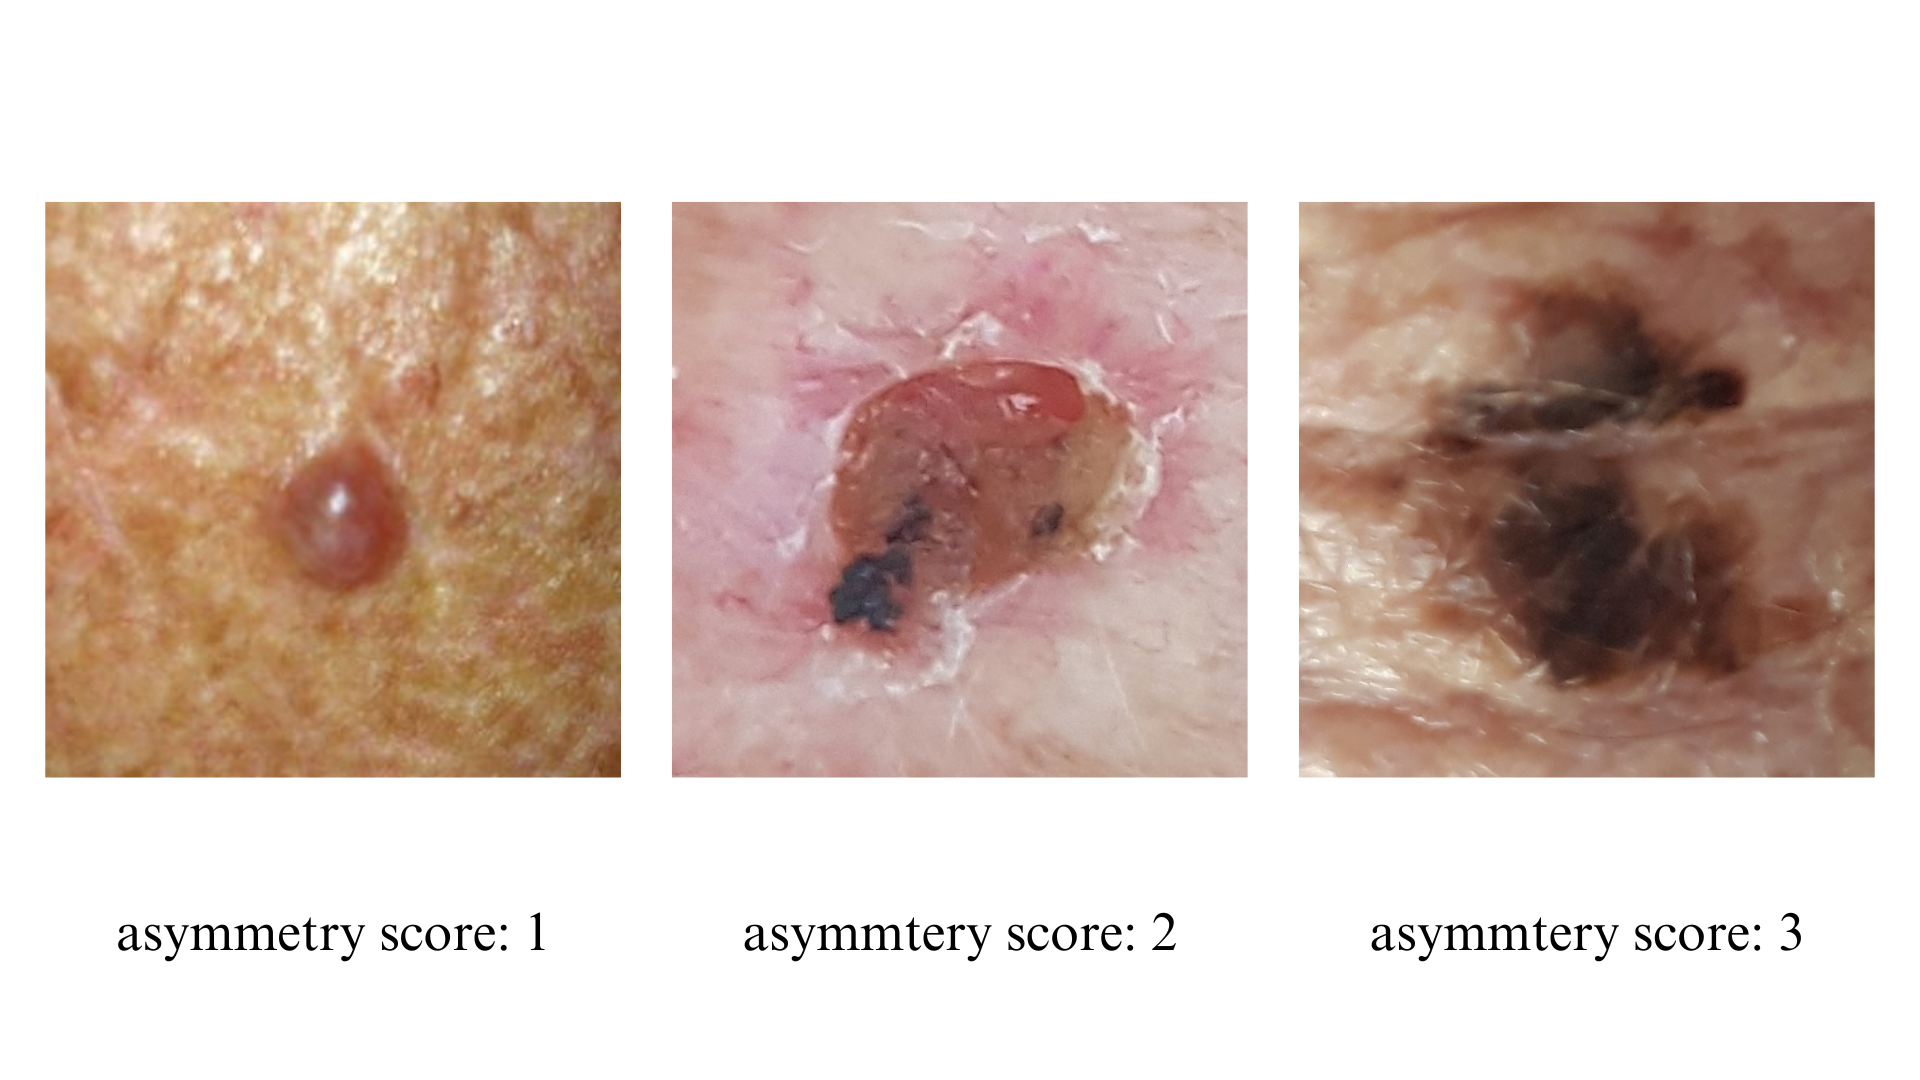
\includegraphics[width=1\linewidth]{asymmetryy.png}
    \caption{Asymmetry score}
    \label{fig:Asymmetry score}
\end{figure}

\begin{figure}[H]
    \centering
    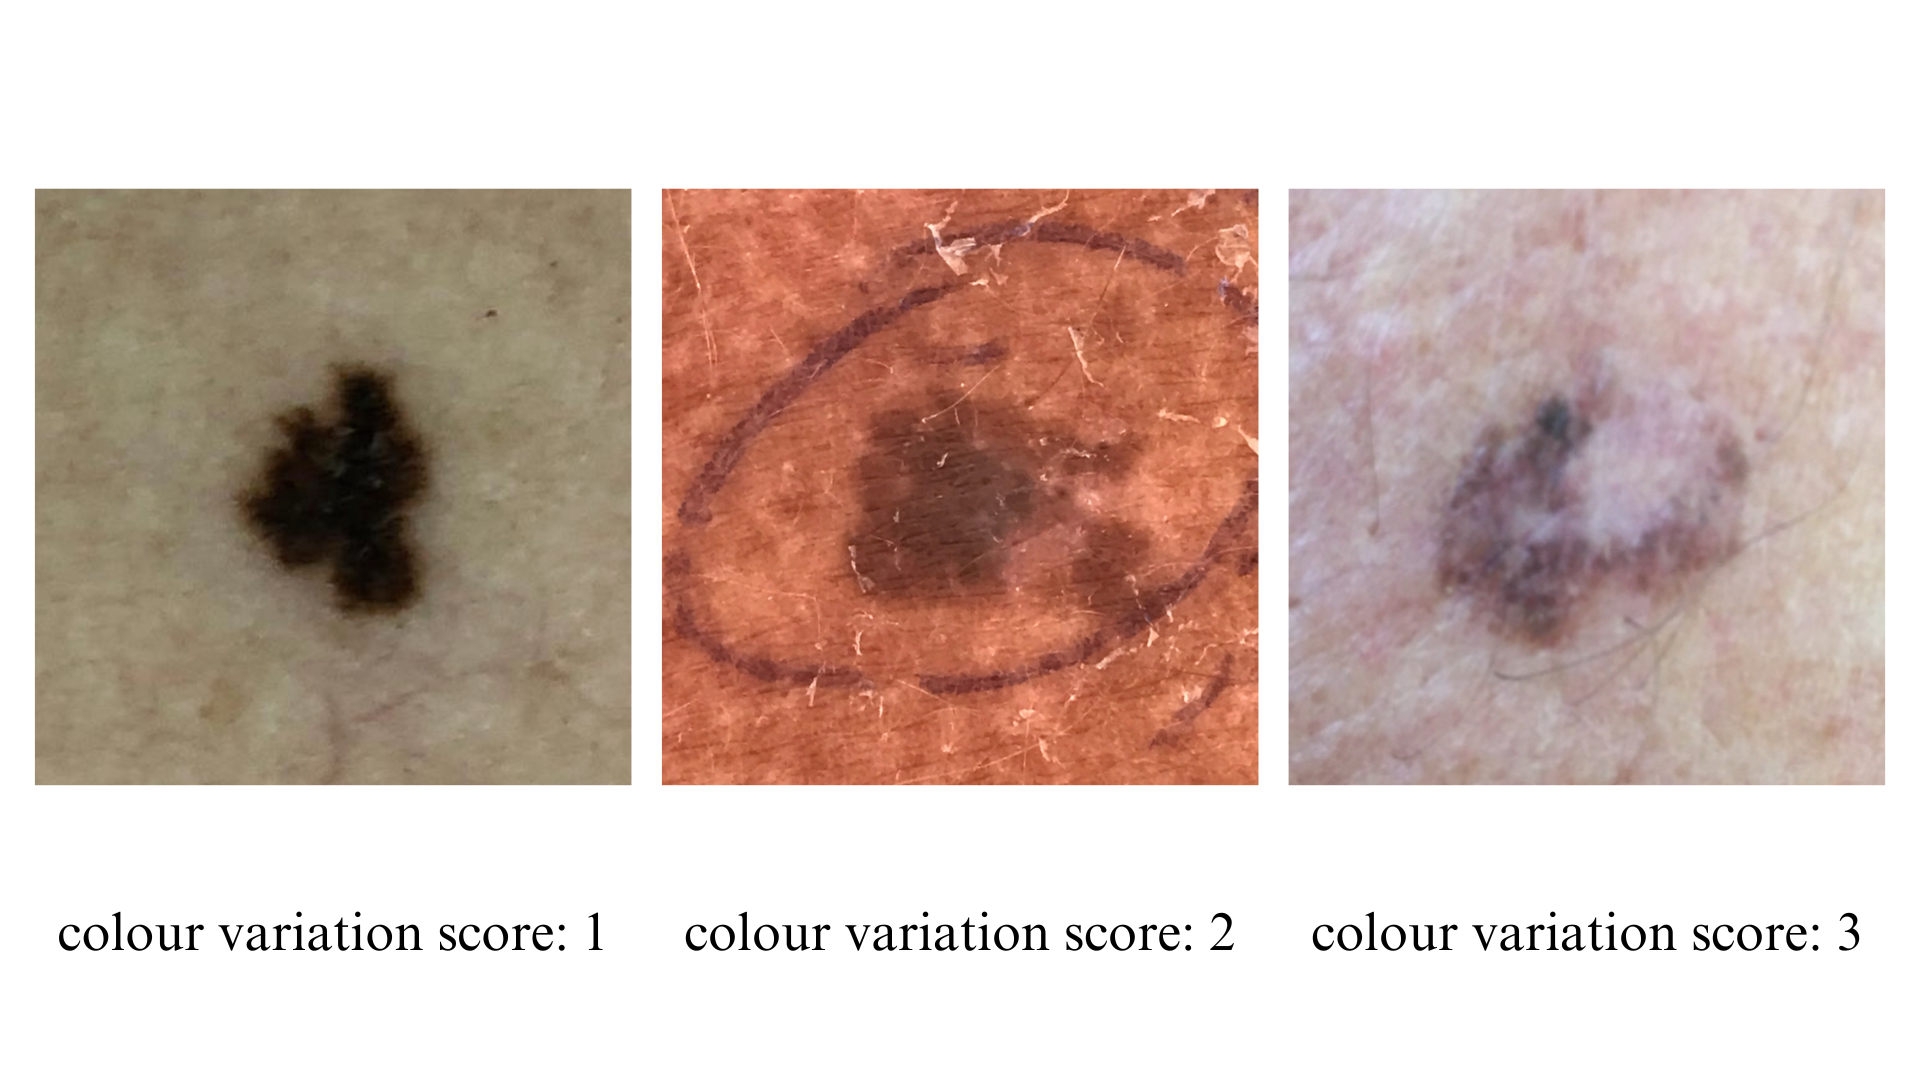
\includegraphics[width=1\linewidth]{colour variation.png}
    \caption{Colour variation score}
    \label{fig:Colour variation score}
\end{figure}

\begin{figure}[H]
    \centering
    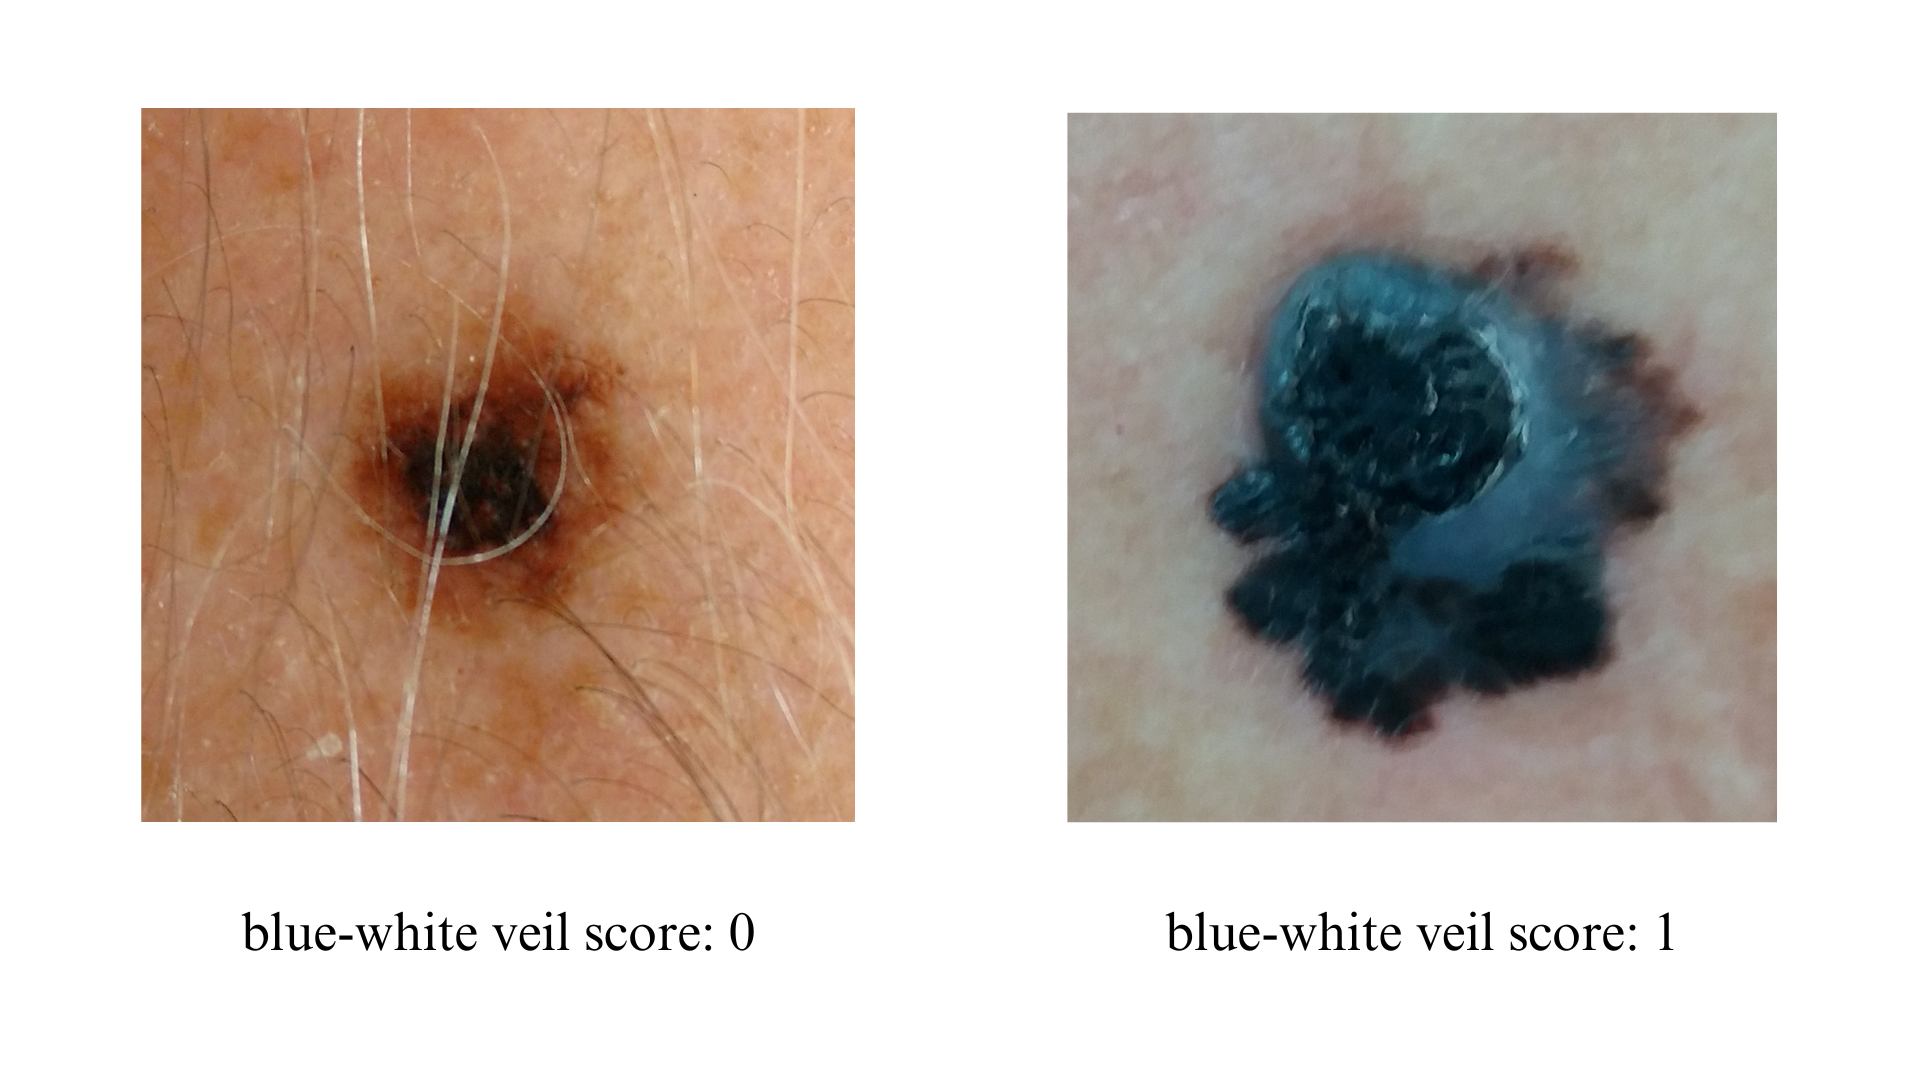
\includegraphics[width=1\linewidth]{blue-white veill.png}
    \caption{Blue-white veil score}
    \label{fig:Blue-white veil score}
\end{figure}

\noindent Based on our manual annotation guide, we gave a score for each of the three features to 120 images (the pictures we created masks for during the first part of the project).
\newline
To apply the scoring system on a larger scale we have written four algorithms to measure the features and segment the lesions.

\subsubsection{Asymmetry}
The algorithm to calculate the asymmetry relies upon a helper function
"FindMajorAxes" which is described below.

\makeatletter
\def\BState{\State\hskip-\ALG@thistlm}
\makeatother
\begin{algorithm}[H]
\caption{FindMajorAxes}
\begin{algorithmic}[1]
\Procedure{FindMajorAxes}{}
\State $major\_axes\_max \gets \text{None}$
\State $mask\_max \gets \text{None}$
\BState \textbf{loop:}
\For{$\text{angle} \gets 0 \text{ to } 180 \text{ by } 10$}
    \State $mask \gets \text{rotate(mask, angle)}$
    \If{$\text{major axes} > major\_axes\_max$}:
        \State $major\_axes\_max \gets \text{major axes}$
        \State $mask\_max \gets \text{mask}$
    \EndIf
\EndFor
\BState \textbf{return} $major\_axes\_max, mask\_max$
\EndProcedure
\end{algorithmic}
\end{algorithm}

\noindent As it can be seen the algorithm rotates a given mask and looks for the largest two axes it can find, compares it to the current largest and updates accordingly. Once the major axes have been found along with the rotation of the mask, the asymmetry index is calculated. The image is folded along the major axes and the overlap is computed to calculate the asymmetry-index.

\[
\text{Asymmetry\_index} = \frac{2 \times |A \cap B|}{|A| + |B|}
\]
where:
\begin{align*}
A & : \text{Overlap along 1st axis} \\
B & : \text{Overlap along 2nd axis} \\
|A| & : \text{Total area lesion} A \\
|B| & : \text{Total area lesion} B \\
|A \cap B| & : \text{Area of the intersection of } A \text{ and } B
\end{align*}

\subsubsection{Colour}
To get a value for the colour variation we are going through the following steps:
\begin{enumerate}
    \item Crop the original image to the size of the lesion in the provided mask:\\
    As we are only interested in the colour variation within the lesion we don't want outside information to influence the rating.
    \item Segment the image into larger "superpixels" and average out the colour:\\
    This is performed by the SLIC ("Simple Linear Iterative Clustering") algorithm, which method uses k-means clustering to create segments with roughly the same colour within the marked area. We average out the colours of these segments to get a uniform value within these.
    \item Convert the image to gray-scale:\\
    We convert the averaged out result to gray-scale to get a single numerical value per segment, we then compare against the other segments. If the values are far apart we can deduct that there are different intensities in the image and thus a higher colour variation and vice versa.
    \item Plot the values to a histogram:\\
    A histogram of such an image represents the distribution of these intensity values. To account for natural variation in the values we summarize the values into a histogram with 30 bins. Given that the colour intensity can vary between 0 and 255 we therefore have a range of 8.5 per column. To filter out any potential noise - e.g. a mask that slightly included also a non lesion part of the image - we take a 95\% interval of the values.
    The values we take from the histogram are the amount of columns that appear in the image, as well as the span between the first and the last column.
\end{enumerate}
The number of columns in the histogram signifies the number of distinct intensity levels present in the image. A larger number of columns implies a greater range of intensities, suggesting more nuanced variations in brightness. A histogram with a broad distribution of columns and diverse spans suggests high colour variation in the image. Conversely, a narrow histogram with clustered columns and limited spans implies a more uniform distribution of intensity values, indicating less variation. 

\begin{figure}[H]
    \centering
    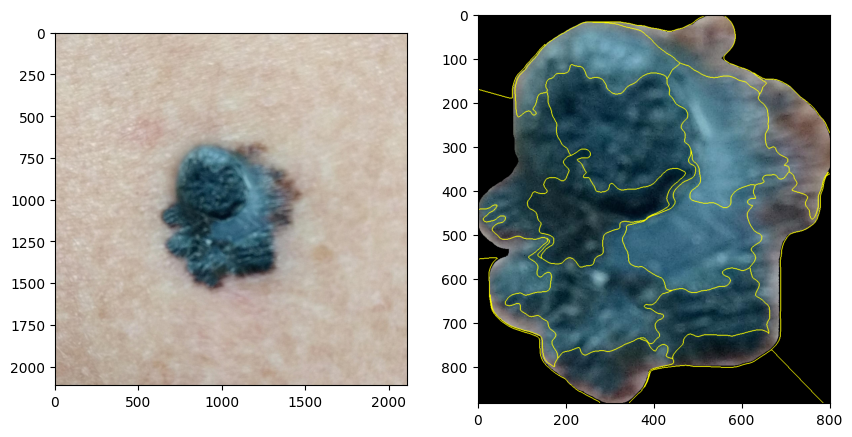
\includegraphics[width=1\linewidth]{Original_Segmentation.png}
    \caption{Original and visualized SLIC segmentations}
    \label{fig:enter-label}
\end{figure}
\begin{figure}[H]
    \centering
    \includegraphics[width=1\linewidth]{Averagecolor_GrayScale.png}
    \caption{Averaged colours and gray-scale}
    \label{fig:enter-label}
\end{figure}

\subsubsection{Blue-White Veil}
In our project, we focused on the detection of blue-white veil in skin lesions, as the extra feature from the 7-point checklist \cite{seven-pointchecklist}.
\newline
The algorithm is designed to process a picture with its corresponding mask. The mask is applied to the image to isolate the lesion, with the rest of the picture set to black.
\newline
After that, we use the SLIC function to segment the lesion based on colour similarity. We get multiple segments of the skin lesion, for each of them we calculate the average RGB values and compare the result to a specific and predefined range of RGB values for blue-white veil. We set this range based on several experiments, especially focused on melanoma pictures, to be in alignment with our expectations on what a blue-white veil should be. If the average colour of a segment is in this range, its area is added to the area of segments containing this feature.
\newline
The final step of the algorithm involves calculating the proportion of the skin lesion affected by blue-white veil by dividing the area of blue-white veil segments with the total area of the lesion. If the value of this proportion is between 20\% and 80\% of the total lesion, it is classified as containing blue-white veil giving a score of 1, and 0 otherwise. We use this criterion in order to guarantee a balanced approach since blue-white veil should cover a significant part of the skin lesion, however not all of it \cite{seven-pointchecklist}.\\
So, the range to determine if a given skin lesion is affected by blue-white veil is: \[20\%\le\frac{\text{area of skin lesion containing blue-white veil}}{\text{total area of skin lesion}}\le80\%\]
\newpage
\noindent The pseudo-code for detecting blue-white veil is the following:

\begin{algorithm}[H]
\caption{Blue-White Veil}
\begin{algorithmic}[1]
\Procedure{Blue-White Veil}{}
\State $segments \gets \text{SLIC}(lesion)$
\State $Area\_bw \gets 0$
\BState \textbf{loop:}
\For{each $segment$ in $segments$}
    \If{$\text{avg\_colour}(segment) \in \text{range\_bw}$}
        \State $Area\_bw \gets Area\_bw + segment$
    \EndIf
\EndFor
\If{$0.2 \leq Proportion\_bw \leq 0.8$}
    \State \Return 1
\Else
    \State \Return 0
\EndIf
\end{algorithmic}
\end{algorithm}

\subsubsection{Segmentation}
In our project, we experimented with three distinct colour-based thresholding methods for segmentation: Otsu's method, mean thresholding, and manual value thresholding. These techniques were selected to outline objects from backgrounds based on intensity levels. However, we encountered inconsistent and unreliable results, particularly when dealing with images featuring varied lighting conditions or complex backgrounds. Additionally, we explored shape-based segmentation techniques, but found their results to be even more inconsistent and less reliable. Consequently, we opted to incorporate manual masks for segmentation, enabling precise definition of objects based on both colour and shape cues. This approach was chosen to enhance the segmentation accuracy and robustness, addressing the limitations observed with solely colour-based methods, especially since the rest of the code in the feature extraction process heavily relied on the masks' quality.

\begin{figure}[H]
    \centering
    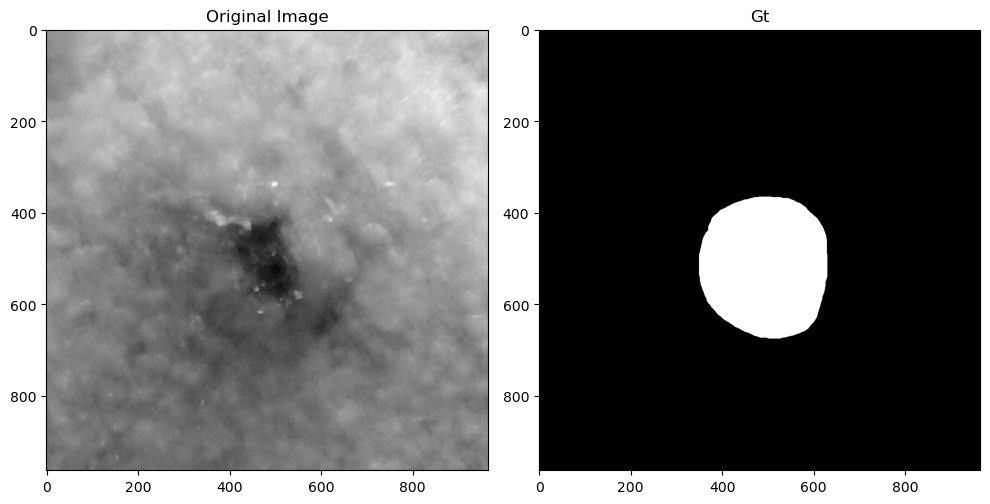
\includegraphics[width=1\linewidth]{original_gt.png}
    \caption{Original image and manual mask}
    \label{fig:enter-label}
\end{figure}
\begin{figure}[H]
    \centering
    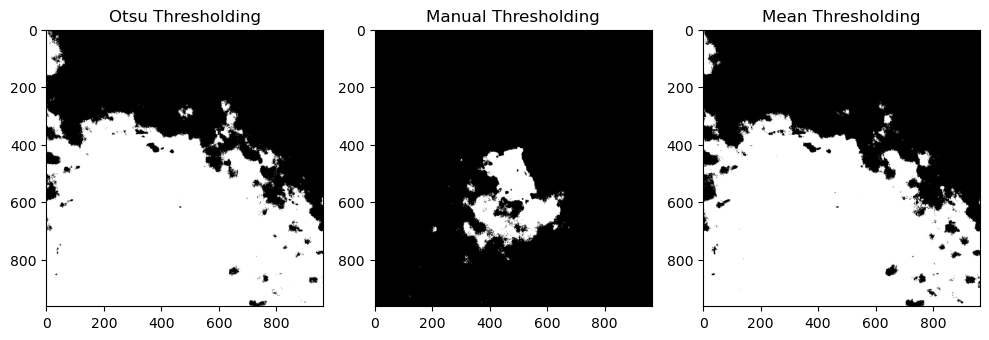
\includegraphics[width=1\linewidth]{result_segmentation.png}
    \caption{Results of automated masking}
    \label{fig:enter-label}
\end{figure}

\section{Experiments}
\input{Experiments}

\section{Results}
The final feature extraction code has been run on 483 pictures among which 51 are melanoma, approximately 10\% of the pictures. 

\subsection{{Classifier selection}}
To find the best classifier, first a k-group split was done on the data, to better help avoid over-fitting and to ensure multiple inputs from the same patients stay in the same group. After splitting up the data, we trained and tested our chosen classifiers on each of the groups and took the average of the results to make a final decision on which classifier to use on the entirety of our data set.
\newline
We have tested 3 different types of classifiers, each with different parameters to find the best one from a total of 12 trained classifiers. After calculating a number of metrics, such as accuracy, area under the ROC curve, sensitivity, etc. we gave the highest importance to sensitivity - as melanoma is a deadly condition and it is important to catch all positive cases - together with the F1 score, which is often used for data sets where the classes are imbalanced, just like in our case with only 10\% melanomas in our data set.

\subsection{{Testing classifiers}}
\textbf{The K-Nearest Neighbours} classifier (KNN) is a non-parametric supervised learning algorithm that classifies an instance based on the majority vote of its k nearest neighbors, using distance metrics such as Euclidean or Manhattan distance, from which we have used sickit-learn’s default setting: the Euclidean distance. We have tested this classifier with K set to 1, 3, 5, and 11. K=1 proved to be the most accurate.
\newline
\textbf{Random Forest} is an ensemble learning method that constructs multiple decision trees during training and outputs the mean prediction (regression) of the individual trees. For this classifier we have experimented with changing both the number of estimators used as well as the maximum possible tree height. A total of 7 classifiers were tested with estimator numbers ranging from 100 to 10,000 and the maximum tree heights from undefined to 10. Of all random forest classifiers, the combination of 10,000 estimators and a maximum height of 5 performed the best.
\newline
\textbf{Logistic Regression} is a statistical method for analysing a data set in which there are one or more independent variables that determine an outcome. It is used to model the probability of a binary outcome based on one or more predictor variables. For this classifier we have used all the default settings of sklearn, no parameters were changed.
Out of all trained classifiers, we have picked the Random Forest classifier with number of estimators set to 10,000 and a maximum tree depth of 5, which averaged a sensitivity score of 0.226, a precision score of 0.517, and an F1 score of 0.303 over the five sets of training data.

\begin{table}[!htb] % Use table* to span both columns
    \caption{Aggregated Results of Classifier Training}
    \begin{tabular}{l c c c} % Adjust column alignment as needed
        \toprule
        & \textbf{Sensitivity} & \textbf{Precision} & \textbf{F1} \\
        \midrule
        KNN & 0.249 & 0.235 & 0.233 \\
        RF & 0.226 & 0.517 & 0.303 \\
        LR & 0.082 & 0.400 & 0.122 \\
        \bottomrule
    \end{tabular}
\end{table}

\subsection{{Results from the trained classifier}}
After running the trained classifier on the entire data set of 483 pictures, we have received that 15 out of the 51 melanomas were correctly identified, which leaves us with 36 false negatives, but no false positives. The 100\% precision sounds like a promising result, however, we would sacrifice that for a higher than 30\% sensitivity score, as that is more a relevant evaluation for detecting melanoma.

\begin{figure}[H]
    \centering
    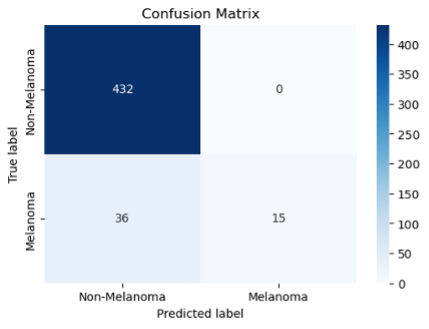
\includegraphics[width=1\linewidth]{ConfusionMatrix.png}
    \caption{Confusion Matrix}
    \label{fig:Confusion Matrix}
\end{figure}

\section{Discussion}
\subsection{Expectations}
The results are mostly in alignment with what could be expected going into this project for several reasons:
\begin{enumerate}
    \item Three features: using only three features for detecting melanoma compared to the usually utilized seven or more is making the process less reliable, especially that one of the features was only present in the data set in very limited cases \cite{seven-pointchecklist}.\
    \item Imbalanced classes: we have worked with almost 500 pictures, but made sure to include all melanoma pictures from the originally available 2,300 pictures, but even so there were only 51 examples for our classifier to work with.\
    \item Limitations in our knowledge: we have learned a lot throughout this project, but it is undeniable that with time and further learning the results can be improved.
\end{enumerate}


\subsection{Possible improvements}
For possible improvements, we consider:
\begin{enumerate}
    \item Feature selection: expanding the feature set beyond just three could enhance the reliability of melanoma detection. Exploring additional relevant features, even if they are not present in every data set, might contribute to a more comprehensive analysis.\

    \item Data augmentation: given the imbalanced classes with only 51 melanoma examples, employing data augmentation techniques could help increase the diversity and quantity of melanoma samples for training the classifier. This involves techniques such as image rotation, flipping, or adding noise to generate synthetic examples.\

    \item Exploring diverse data sets: incorporating additional data sets containing diverse melanoma images provide a more comprehensive understanding of melanoma characteristics and aid in improving the classifier's performance. Accessing varied data sets sourced from different sources or demographics could help address limitations in our current data set and contribute to more robust model training.\

    \item Adjusting the threshold: while our current model operates with a 50\% threshold for melanoma classification, there's potential for refinement. By balancing the precision with prioritizing fewer false negatives over false positives, we can fine-tune the accuracy-precision trade-off. This strategic optimisation of the threshold parameter holds promise for improved classification outcomes. Thus, future iterations of our model could benefit from a systematic exploration of alternative threshold settings, potentially enhancing our accuracy for melanoma.
    
\end{enumerate}

\section{Conclusion}
An important aspect to consider is that melanoma is typically classified based on more available data, such as the patient data combined with neural networks \cite{pacheco2020padufes} or based on the 7 features \cite{seven-pointchecklist}, among which blue-white veil is one of them. However, we are trying to correctly classify melanoma based on a limited number of features compared to the amount typically used, which shows in the results.\\
\newline
Another aspect to consider is the limitations of our coding abilities. Upon initial inspection of the images, we discovered irregular blotches in many melanoma pictures. Coding the automatic feature extractor for this feature proved close to impossible, with very limited reference material on the internet. Blue-white veil was, as shown, a feature not present in many pictures; however, it was possible to detect automatically.\\
\newline
Overall it will be difficult to use the trained classifier in the real world, as the random forest classifier resulted in 70\% of false negatives. For a life threatening disease such as melanoma, this outcome could be detrimental. The chosen three features (colour, asymmetry and blue-white veil) do therefore not seem feasible for this data set to safely classify melanoma.

\bibliographystyle{acl}
\bibliography{acl2015}

\end{document}